\chapter[Time Value of Money]{Time Value of Money (10\%-15\%)}

\subsection{Information}

\begin{distributions}[Objective]
The Candidate will understand and be able to perform calculations relating to present value, current value, and accumulated value.
\end{distributions}

\begin{outcomes}[Learning outcomes]
The candidate will be able to:
\begin{enumerate}[label = \alph*), leftmargin = *]
	\item	Define and recognize the \textit{definitions} of the following terms:
		\begin{itemize}[leftmargin = *]
		\item	Interest rate (rate of interest);
		\item	Simple interest;
		\item	Compound interest;
		\item	Accumulation function;
		\item	Future value;
		\item	Current value;
		\item	Present value;
		\item	Net present value;
		\item	Discount factor;
		\item	Discount rate (rate of discount);
		\item	Convertible $m$-thly (\dots ?);
		\item	Nominal rate;
		\item	Effective rate;
		\item	Inflation;
		\item	Real rate of interest;
		\item	Force of interest;
		\item	Equation of value.
		\end{itemize}
	\item	Given any 3 of:
		\begin{itemize}[leftmargin = *]
		\item	Interest rate;
		\item	Period of time;
		\item	Present value;
		\item	Current value;
		\item	Future value,
		\end{itemize}
		calculate the remaining item using \textit{simple} or \textit{compound} interest;
	\item[]	Solve time value of money equations involving variable force of interest;
	\item	Given any 1 of:
		\begin{itemize}[leftmargin = *]
		\item	Effective interest rate;
		\item	Nominal interest rate convertible $m$-thly;
		\item	Force of interst,
		\end{itemize}
		calculate any of the other items;
	\item	Write the equation of value given a set of cash flows and interest rate.
\end{enumerate}
\end{outcomes}

\begin{ASM_chapter}[Related lessons ASM]
Section 1: Interest rates and Discount Rates
\begin{itemize}[leftmargin = *]
	\item	\nameref{L.-1a}
	\item	\nameref{L.-1b}
	\item	\nameref{L.-1c}
	\item	\nameref{L.-1d}
	\item	\nameref{L.-1e}
	\item	\nameref{L.-1f}
	\item	\nameref{L.-1g}
	\item	\nameref{L.-1h}
\end{itemize}
Section 2: Practical Applications
\begin{itemize}[leftmargin = *]
	\item	\nameref{L.-2a}
	\item	\nameref{L.-2b}
\end{itemize}
\end{ASM_chapter}

\subsection{Chapter summaries}

\begin{CHPT_SUMM_AUTO}[label = {L.-1a}]{1a. Basic Concepts}
\begin{FORMULA_SUMM}{Effective rate of interest}
\begin{description}
	\item[$a(t)$]	\textbf{Accumulation function} defined as the Accumulated Value (AV) of the fund at time $t$ of an initial investment of $\$1.00$ at time 0.
		\begin{itemize}[leftmargin = *]
		\item	$a(0) \equiv 1$.
		\item	Generally \textbf{continuous} and \textbf{increasing}.
		\end{itemize}
	\item[$a(t) - a(t - 1)$]	\textbf{\textit{Amount} of growth} in the $t^{\text{th}}$ year.
		\begin{itemize}[leftmargin = *]
		\item	a.k.a. the interest earned
		\end{itemize}
	\item[$\frac{a(t) - a(t - 1)}{a(t - 1)}$]	\textbf{\textit{Rate} of growth} in the $t^{\text{th}}$ year.
		\begin{itemize}[leftmargin = *]
		\item	a.k.a. effective rate of interest denoted $i_{t}$.
		\end{itemize}
	\item[$A(t)$]	\textbf{Amount function} defined as the Accumulated Value (AV) of the fund at time $t$ of an initial investment of $\$k$ at time 0.
		\begin{itemize}[leftmargin = *]
		\item	$A(t) = k a(t)$.
		\end{itemize}
	\item[$i_{t}$]	\textbf{Effective rate of interest} defined as the rate of growth based on the amount in the fund at the \textbf{\textit{beginning}} of the year.
		\begin{itemize}[leftmargin = *]
		\item	$i_{t} = \frac{A(t) - A(t - 1)}{A(t - 1)}$.
		\item	We deduce $A(t) = (1 + i_{t})A(t - 1)$.
		\end{itemize}
\end{description}
\end{FORMULA_SUMM}

\begin{FORMULA_SUMM}{Effective Rate of Discount}
\begin{description}
	\item[$d_{t}$]	\textbf{Effective rate of discount} defined as the rate of growth based on the amount in the fund at the \textbf{\textit{end}} of the year.
		\begin{itemize}[leftmargin = *]
		\item	$d_{t} = \frac{A(t) - A(t - 1)}{A(t)}$.\
		\item	Although we could get by without it, it's useful to determine the amount to pay today for a specified amount in the future.
		\end{itemize}
	\item[Discounting]	Finding the price we'd be willing to pay for the promise to receive a future amount.
		\begin{itemize}[leftmargin = *]
		\item	a.k.a. finding the present value which is why $i = \frac{d}{1 - d}$.
		\item	$v = (1 - d) = \frac{1}{1 + i}$.
		\item	$d = \frac{i}{1 + i}$.
		\end{itemize}
\end{description}
\end{FORMULA_SUMM}

\begin{FORMULA_SUMM}{Nominal Rates of Interest}
\begin{description}
	\item[$i^{(m)}$]	\textbf{Nominal} annual rate of of interest \textbf{compounded $m$ times a year}.
	\item[$\frac{i^{(m)}}{m}$]	\textbf{Effective} rate of of interest \textbf{for an $m^{\text{th}}$ of a year}.
		\begin{itemize}[leftmargin = *]
		\item	Thus $(1 + i) = \left(1 + \frac{i^{(m)}}{m}\right)^{m}$.\
		\end{itemize}
\end{description}
\end{FORMULA_SUMM}
\end{CHPT_SUMM_AUTO}

\begin{CHPT_SUMM_AUTO}[label = {L.-1b}]{1b. Why Do We Need a Force of Interest?}
	\begin{itemize}[leftmargin = *]
		\item	An effective rate of interest gives information about both the starting and ending values but none on the value in between.
		\item	In contrast, the force of interest can give information \textbf{at any given time} about the rate of growth.
		\item	The plot of four different funds' growth curves (with both the same starting and ending values) is a perfect visualization:
		\begin{center}
			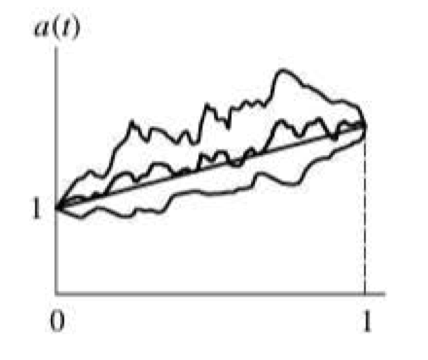
\includegraphics[scale=0.6]{img/annuities-force.png}
		\end{center}
	\end{itemize}
\end{CHPT_SUMM_AUTO}

\begin{CHPT_SUMM_AUTO}[label = {L.-1c}]{1c. Defining the Force of Interest}
	\begin{itemize}[leftmargin = *]
		\item	To obtain a rate of growth \textit{proportional to the amount invested}, the derivative is divided by the amount function.
		\item	Two funds can have the same rate of change but different amounts originally invested.
		\item	In this case, the fund growing with the smaller amount of money actually a \textit{smaller} rate of change.
	\end{itemize}
	
\paragraph{TRAP} If given the derivative of the accumulation function, $a'(t)$, use the property that the fund at the beginning is 1, $a(0) = 1$, to define the $+ C$ when integrating for $a(t)$.
\end{CHPT_SUMM_AUTO}

\begin{CHPT_SUMM_AUTO}[label = {L.-1d}]{1d. Finding the Fund in Terms of the Force of Interest}
	\begin{itemize}[leftmargin = *]
		\item	If we want to find the accumulation, or amount, function from the force of interest we inverse the equation.
		\item	To do so, recall that $\frac{\partial}{\partial x}\ln(f(x)) = \frac{f'(x)}{f(x)}$.
		\item	Also $\int_{0}^{t} \frac{\partial}{\partial r} \ln(a(r)) dr = 	\ln(a(r))\big|_{0}^{t} =	\ln(a(t))$.
	\end{itemize}
	
\begin{FORMULA_SUMM}{Force of interest}
\begin{description}
	\item[Force of interest]	the rate of growth at a point in time.
		\begin{itemize}[leftmargin = *]
		\item	a.k.a. finding the present value which is why $i = \frac{d}{1 - d}$.
		\item	$v = (1 - d) = \frac{1}{1 + i}$.
		\item	$d = \frac{i}{1 + i}$.
		\end{itemize}
	\item[$\delta_{t}$]	The \textbf{Force of interest} at time $t$.
		\begin{itemize}[leftmargin = *]
		\item	$\delta_{t} = \frac{A'(t)}{A(t)}$.
		\item	$a(t)	=	\textrm{e}^{\int_{0}^{t}\delta_{r}dr}$
		\end{itemize}
\end{description}
\end{FORMULA_SUMM}
\end{CHPT_SUMM_AUTO}

\begin{CHPT_SUMM_AUTO}[label = {L.-1e}]{1e. The Simplest Case: A Constant Force of Interest}

\begin{FORMULA_SUMM}{Simple Force of interest}
\begin{description}
	\item[$\delta$]	The constant force of interest.
		\begin{itemize}[leftmargin = *]
		\item	a.k.a. the nominal rate of interest compounded continuously.
		\item	$\delta = \underset{m \rightarrow \infty}{\lim} i^{(m)} = i^{(\infty)} = \ln(1 + i)$.
		\item	$a(t)	=	\textrm{e}^{\int_{0}^{t}\delta dr}	=	\textrm{e}^{\delta t}$.
		\end{itemize}
\end{description}
\end{FORMULA_SUMM}
\end{CHPT_SUMM_AUTO}

\begin{CHPT_SUMM_AUTO}[label = {L.-1f}]{1f. Power Series}
	\begin{itemize}[leftmargin = *]
		\item	Not really on past exams, section is \og just in case \fg{}.
	\end{itemize}
\end{CHPT_SUMM_AUTO}

\begin{CHPT_SUMM_AUTO}[label = {L.-1g}]{1g. The Variable Force of Interest Trap}
	\begin{itemize}[leftmargin = *]
		\item	When we want the accumulated value of an amount not invested at the beginning, we integrate the force of interest over the respective integral. 
		\item	Alternatively, we can take the ratio of the accumulation function at both times.
	\end{itemize}

\begin{FORMULA_SUMM}{Variable Force of interest}
\begin{align*}
	FV
	&=	\textrm{e}^{\int_{t_{1}}^{t_{2}}\delta_{r} dr}	\\
	&\equiv	\frac{a(t_{2})}{a(t_{1})}	
\end{align*}
\end{FORMULA_SUMM}
\end{CHPT_SUMM_AUTO}

\begin{CHPT_SUMM_AUTO}[label = {L.-1h}]{1h. Equivalent Rates}
	\begin{itemize}[leftmargin = *]
		\item	
	\end{itemize}
\end{CHPT_SUMM_AUTO}

\begin{CHPT_SUMM_AUTO}[label = {L.-2a}]{{2a. Equations of Value, Time Value of Money, and Time Diagrams}}
\begin{description}
	\item[Time value (equivalence principle)]	1\$ today is not equivalent to 1\$ a year from now. However, 1\$ today is equivalent to 1.05\$ a year from now if the rate of interest is 5\%. 
	\item[Comparison date]	Date at which we solve the \textbf{equation of of value}.
\end{description}
	\begin{itemize}[leftmargin = *]
		\item	Important to use \textbf{time lines} to solve problems:
		\begin{center}
		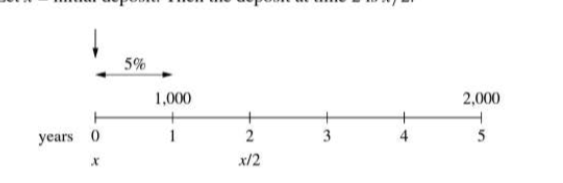
\includegraphics[scale=0.4]{img/time-value-timeline.png}
		\end{center}
		\item	We can treat a problem by \textbf{payment} or \textbf{interest} period.
	\end{itemize}
\end{CHPT_SUMM_AUTO}

\begin{CHPT_SUMM_AUTO}[label = {L.-2b}]{2b. Unknown Time and Unknown Interest Rate}
	\begin{itemize}[leftmargin = *]
		\item	Can approximate the time $\bar{t}$ by using a weighted average of the time of payment times the amount of payment divided by the total amount paid with the \textbf{method of equated time}. For example:
		\begin{center}
		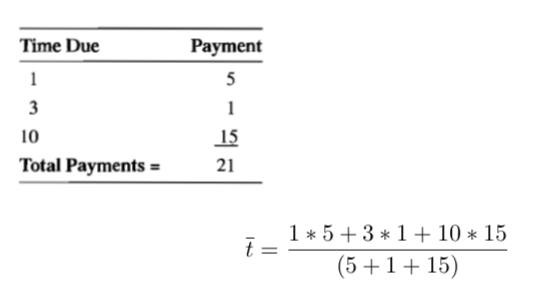
\includegraphics[scale=0.5]{img/approx-time-pmt.png}
		\end{center}
	\end{itemize}
\end{CHPT_SUMM_AUTO}
